%\documentclass{pbml}
\documentclass[nofonts]{pbml} % use default fonts
%\documentclass[color]{pbml} % for color images and hypertext links

\usepackage{graphicx}
\usepackage{multicol}
\usepackage{amssymb}
\usepackage{natbib}
\usepackage{euler}
\usepackage{latexsym}
\usepackage{verbatim}
\usepackage{amsmath}
\usepackage{tikz}
\usepackage{wrapfig}
\usepackage{colortbl}
\usepackage{xcolor}
\usepackage{hyperref}
\usepackage{qtree}
\usetikzlibrary{fit,positioning}

\hypersetup{
    colorlinks=false,
    pdfborder={0 0 0},
}

\newcommand{\ensuretext}[1]{#1}
\newcommand{\mycomment}[3]{\ensuretext{\textcolor{#3}{[#1 #2]}}}
\newcommand{\ammarker}{\ensuretext{\textcolor{blue}{\ensuremath{^{\textsc{A}}_{\textsc{M}}}}}}
\newcommand{\am}[1]{\mycomment{\ammarker}{#1}{blue}}
\newcommand{\cjmarker}{\ensuretext{\textcolor{red}{\ensuremath{^{\textsc{C}}_{\textsc{D}}}}}}
\newcommand{\cjd}[1]{\mycomment{\cjmarker}{#1}{red}}
\newcommand{\ignore}[1]{}
\newcolumntype{C}{>{\centering\arraybackslash}p{0.6ex}}

\begin{document}
\title{Tree Transduction Tools for cdec}

\institute{label1}{Carnegie Mellon University}
\institute{label2}{University of Oxford}

\author{
  firstname=Austin,
  surname=Matthews,
  institute=label1,
}
\author{
  firstname=Paul,
  surname=Baltescu,
  institute=label2,
}
\author{
  firstname=Phil,
  surname=Blunsom,
  institute=label2,
}
\author{
  firstname=Alon,
  surname=Lavie,
  institute=label1,
}
\author{
  firstname=Chris,
  surname=Dyer,
  institute=label1,
  corresponding=yes,
  email={cdyer@cs.cmu.edu},
  address={Language Technologies Institute\\Carnegie Mellon University\\Pittsburgh, PA 15213, United States}
}

\PBMLmaketitle

\begin{abstract}
We describe a collection of open source tools for learning
tree-to-string and tree-to-tree transducers and the extensions to the
cdec decoder that enable translation with these. Our modular,
easy-to-extned tools extract rules from trees or forests aligned to
strings and trees subject to different structural constraints. A fast,
multithreaded implementation of the Cohn and Blunsom (2009) model for
extracting compact tree-to-string rules is also included. The
implementation of the tree composition algorithm used by cdec is
described, and translation quality and decoding time results are
presented. Our results add to the body of evidence suggesting that
tree transduers are a compelling option for translation, particularly
when decoding speed and translation model size are important.
\end{abstract}

%\section{Introduction}

%\section*{Acknowledgements}
%This research is supported by \ldots

\section{Tree to String Transducers}
Tree-to-string transducers that define relations on strings and trees are a popular formalism for capturing translational equivalence where syntactic tree structures are available in either the source or target language \citep{graehl:2008,Galley2004,rounds:1970,thatcher:1970}. The tools described in this paper are a restricted version of top-down tree transducers that support multi-level tree fragments on one side and strings on the other, with no copying or deletion \citep{huang:2006,Cohn2009}. Such transducers can elegantly capture syntactic regularities in translation. For example see Fig.~\ref{fig:exxrs}, which gives the rules necessary to translate between English (an SVO language with ditransitive verbs) and Welsh (a VSO language with prepositional datives).
\begin{figure}[t]
\vspace{-.4cm}
\begin{minipage}[t]{0.45\linewidth}
\begin{small}
\vspace{-.5cm}\begin{align*}
\textrm{(S \fbox{NP} (VP \fbox{VBD} \fbox{NP} \fbox{NP}))} &\leftrightarrow \scriptsize{\fbox{2}}\ \scriptsize{\fbox{1}}\ \scriptsize{\fbox{4}} \ \textrm{\emph{i} } \scriptsize{\fbox{3}} \\
\textrm{(NP (DT \emph{a}) \fbox{NN})}  &\leftrightarrow  \scriptsize{\fbox{1}} \\
\textrm{(VBD \emph{gave})}& \leftrightarrow \textrm{\emph{rhoddodd}} \\
\textrm{(NN \emph{book}))} &\leftrightarrow \textrm{\emph{lyfr}} \\
\textrm{(NP (PRP \emph{me}))} &\leftrightarrow \textrm{\emph{mi}} \\
\textrm{(NP (NNP John))} &\leftrightarrow \textrm{\emph{Ioan}}
\end{align*}
\end{small}
\end{minipage}
\hspace{0.3cm}
\begin{minipage}[t]{0.45\linewidth}
\begin{small}
\Tree  [.S [.NP [.NNP \emph{John} ] ] [.VP [.VBD \emph{gave} ] [.NP [.PRP \emph{me} ] ] [.NP [.DT \emph{a} ] [.NN \emph{book} ] ] ] ]
\end{small}
\end{minipage}

\vspace{+0.4cm} {\tt cdec} text format of above transducer (with example features):
\begin{small}
\begin{verbatim}
  (S [NP] (VP [VBD] [NP] [NP])) ||| [2] [1] [4] i [3] ||| logP(s|t)=-0.2471
  (NP (DT a) [NN]) ||| [1] ||| logP(s|t)=-0.6973 Delete_a=1
  (VBD gave) ||| rhoddodd ||| logP(s|t)=-2.3613
  (NN book) ||| lyfr ||| logP(s|t)=-0.971
  (NP (PRP me)) ||| mi ||| logP(s|t)=-1.3688
  (NP (NNP John)) ||| Ioan ||| logP(s|t)=0
\end{verbatim}
\end{small}
\vspace{+0.5cm}{\tt cdec} input text format of above tree:
\begin{small}
\begin{verbatim}
  (S (NP (NNP John)) (VP (VBD gave) (NP (PRP me)) (NP (DT a) (NN book))))
\end{verbatim}
\end{small}

\caption{\label{fig:exxrs}Example single-state transducer that transduces between the SVO English tree (upper right of figure) and its VSO Welsh translation: \emph{rhoddodd Ioan lyfr i mi}.}
\end{figure}
\begin{figure}
\begin{small}
\begin{align*}
q_0 : \textrm{(S \fbox{NP} (VP \fbox{VB} \fbox{NP}))} &\leftrightarrow \scriptsize{\fbox{1}}:q_0\ \scriptsize{\fbox{2}}:q_0\ \scriptsize{\fbox{3}}:q_{\textrm{\emph{acc}}} \\
q_0 : \textrm{(NP (DT \emph{the}) \fbox{NN})} &\leftrightarrow \textrm{\emph{der }}  \scriptsize{\fbox{1}}:q_0 \\
q_{\textrm{\emph{acc}}} : \textrm{(NP (DT \emph{the}) \fbox{NN})} &\leftrightarrow \textrm{\emph{den }}  \scriptsize{\fbox{1}}:q_0 \\
q_0 : \textrm{(NN \emph{dog})} &\leftrightarrow \textrm{\emph{Hund}}
\end{align*}
\end{small}
{\tt cdec} text format of above transducer (with example features):
\begin{small}
\begin{verbatim}
  [Q0] ||| (S [NP] (VP [VB] [NP])) ||| [Q0,1] [Q0,2] [QACC,3] ||| lp=-2.9713
  [Q0] ||| (NP (DT the) [NN]) ||| der [Q0,1] ||| lp=-1.3443
  [QACC] ||| (NP (DT the) [NN] ||| den [Q0,1] ||| lp=-2.9402
  [Q0] ||| (NN dog) ||| Hund ||| lp=-0.3171
\end{verbatim}
\end{small}
\caption{\label{fig:multistate}A tree-to-string transducer with multiple states encoding structural information for choosing the proper nominal inflection in English--German translation.}
\end{figure}
In our notation, transducers consist of a set of rules (also called edges) which pair a tree fragment in one language with a string of terminal symbols and variables in a second language. Frontier nonterminal nodes in the tree fragment are indicated with a box around the nonterminal symbol, and the corresponding substitution site in the string is indicated by a box around a number indexing the nonterminal variable in the tree fragment (counting in top-down, left to right, depth first order). Additionally, tree-to-string transducers can be further generalized so as to have multiple transducer states, shown in Fig.~\ref{fig:multistate}. The transducers in Fig.~\ref{fig:exxrs} can be understood to have a single state. For formal properties of tree-to-string transducers, we refer the reader to the above citations. 

Tree-to-string transducers define a relation on strings and trees and, in translation applications, are capable of transforming either source trees (generated by a parser) into target language strings or source strings into target language parsers. Running the transducer in the tree-to-string direction can avail itself of specialized algorithms similar to finite state composition (\S\ref{sec:cdec}); in the string-to-tree direction, they can be trivially converted to synchronous context free grammars and transduction can be carried out with standard CFG parsing algorithms \citep{Galley2004}.

\section{Tree-to-string translation with {\tt cdec}}
\label{sec:cdec}

The {\tt cdec} decoder \citep{Dyer_etal_2010} has a modular decoder architecture that factors the decoding problem into multiple stages: first, a hypergraph is generated that represents the translation search space produced by composing the input (a string, lattice, or tree) with the relevant transducer (a synchronous context-free grammar, a finite state transducer, etc.); second, the hypergraph is rescored---and possibly restructured (in the case of adding an $n$-gram language model)---with generic feature extractors; finally, various outputs of interest are extracted (the best translation, the $k$-best translations, alignments to a target string, statistics required for parameter optimization, etc.).

The original {\tt cdec} implementation contained hypergraph generators based on a variety of translation backends, although SCFG translation is the most widely used \citep{chiang:2007}. In this section, we describe the tree-to-string algorithm that generates a translation forest given a source language parse tree and a tree-to-string transducer.

The construction of the hypergraph takes place by composing the input tree with the tree-to-string transducer using a top down, recursive algorithm. Intuitively, the algorithm matches all rules in the transducer that start at a given node in the input tree and match at least one complete rewrite in the source tree. Any variables that were used in the match are then recursively processed until the entire input tree is completed. To make this process efficient, the tree side of the input transducer is determinized by depth-first, left-to-right factoring---this process is analogous to left factoring a context-free grammar \citep{klein:2001}. By representing the tree using the same depth-first, left-to-right representation, standard DFA intersection algorithms can be used to compute each step of the recursion. The DFA representation of a transducer (tree side) and an input tree (starting at nonterminal S) is shown in Fig.~\ref{fig:det}.

\begin{figure}[t]
\centering
\includegraphics[scale=0.5]{tree-as-dfa.pdf}
\caption{\label{fig:det}DFA representation of a tree transducer (above) and an input tree (middle). This transducer will transduce the input tree to the hypergraph (below) yielding a single string \emph{x y z}, using rules (r1) and (r3). Red octagons are closing parentheses.}
\end{figure}

To understand how this algorithm procedes on this particular input, the input tree DFA is matched against the `S' DFA. The output transductions are stored in the final states of the transducer DFA, and when a path is matched, an edge is added to the output hypergraph, one per matched path per translation option. Variables that were used in the input are then recursively processed, starting from the relevant transducer DFA (in this case, the `A' DFA will be invoked recursively).

\section{Bayesian Synchronous Tree to String Grammar Induction}
\label{sec:bayes}

In this section, we present an open source implementation of the synchronous tree-to-string grammar induction algorithm proposed by \citet{Cohn2009} \footnote{Our code is publicly available here: \url{https://github.com/pauldb89/worm}}. This algorithm relies on a Bayesian model which incorporates a prior preference for learning small, generalizable STSG rules. The model is designed to jointly learn translation rules and word alignments. This is important for capturing long distance reordering phenomena, which might otherwise be ignored if the rules are inferred using distance penalized alignments (e.g. as in the heuristic proposed by \citet{Galley2004}).

The model represents the tree-to-string grammar as a set of distributions $\{G_c\}$ over the productions of each non-terminal $c$. Each distribution $G_c$ is assumed to be generated by a Dirichlet Process with a concentration parameter $\alpha_c$ and a base distribution $P_0(\cdot \mid c)$, i.e. $G_c \sim DP(\alpha_c, P_0(\cdot \mid c))$. The concentration parameter $\alpha_c$ controls the model's tendency towards reusing rules or creating new ones according to the base distribution and has a direct influence on the size of the resulting grammar. The base distribution is defined to assign probabilities to an infinite set of rules. The probabilities decrease exponentially as the sizes of the rules increase, biasing the model towards learning smaller rules.

Instead of representing the distributions $G_c$ explicitly, we integrate over all the possible values of $G_c$. We obtain the following formula for estimating the probability of a rule $r$ with root $c$, given a fixed set of derivations $\textbf{r}$ for the training corpus:
\begin{equation}
p(r \mid \textbf{r}, c; \alpha_c, P_0) = \frac{n_{r} + \alpha_c P_0(r \mid c)}{n_{c} + \alpha_c},
\label{eq:sampling}
\end{equation}
where $n_{r}$ is the number of times $r$ occurs in $\textbf{r}$ and $n_{c}$ is the number of rules with root $c$ in $\textbf{r}$.

\citet{Cohn2009} train their model using Gibbs sampling. To simplify the implementation, an alignment variable is defined for every internal node in the parsed corpus. An alignment variable specifies the interval of target words which are spanned by a source node. Alternatively, a node may not be aligned to any target words or may span a discontiguous group of words, in which case it is annotated with an empty interval. Non-empty alignment variables mark the substitution sites for the rules in a derivation of a parse tree. Overall, they are used to specify a set of sampled derivations $\textbf{r}$ for the entire training data. Alignment spans are constrained to subsume the spans of their descendants and must be contained within the spans of their ancestors. In addition to this, sibling spans belonging to the frontier of the same rule must not overlap.

We implement Gibbs sampling with the help of two operators: \texttt{expand} and \texttt{swap}. The \texttt{expand} operator works by resampling a randomly selected alignment variable $a$, while keeping all the other alignment variables fixed. The set of possible outcomes consists of the empty interval and all the intervals assignable to $a$ such that the previous conditions continue to hold. Each outcome is scored proportionally to the new rules it creates,  using \autoref{eq:sampling}, conditioned on all the rules in the training data that remain unaffected by the sampling operation. The \texttt{swap} operator randomly selects two frontier nodes labelled with non-terminals belonging to the same STSG rule and chooses to either swap their alignment variables or to leave them unchanged. The outcomes are weighted similarly to the previous case. The goal of the \texttt{swap} operator is to improve the sampler's ability to mix, especially in the context of improving word reordering, by providing a way to execute several low probability \texttt{expand} steps at once.

Our implementation of the grammar induction algorithm is written in \texttt{C++}. Compiling the code results in several binaries, including \texttt{sampler}, which implements our Gibbs sampler. The grammar induction tool expects the following as input:
\begin{itemize}
\item A file containing the parse trees for the source side of the parallel corpus, in the Penn Treebank format.
\item A file containing the target side of the parallel corpus.
\item A file containing the word alignments for the training data. The word alignments are needed in the heuristic \citep{Galley2004} used to initialize the first set of derivations.
\item Two files containing the translation tables $p(s \mid t)$ and $p(t \mid s)$. These probabilities are used in the base distribution to weight the rules according to the source and target words they contain.
\end{itemize}
The remaining input arguments (hyperparameters, rule restrictions, etc.) are initialized with sensible default values. Running the binary with the \texttt{-{}-help} option will produce the complete list of arguments and a brief explanation for each. The tool produces several files as output, including one containing the set of rules together with their probabilities, computed based on the last set of sampled derivations. The documentation released with our code shows how to prepare the training data, run the tool and convert the output in the \texttt{cdec} format.
/github

Our tool leverages the benefits of a multithreaded environment to speed up grammar induction. At every sampler iteration, each training sentence is dynamically allocated to one of the available threads. In our implementation, we use a hash-based implementation of a Chinese Restaurant Process (CRP) \citep{Teh2010} to efficiently compute the rule probabilities given by \autoref{eq:sampling}. The data structure is updated whenever one of the \texttt{expand} or \texttt{swap} operators is applied. To lock this data structure with every update would completely cancel the effect of parallelization, as all the basic operations performed by the sampler are dependent on the CRP. Instead, we distribute a copy of the CRP on every thread and synchronize the data structures at the end of each iteration. Although the CRPs diverge during an iteration through the training data, no negative effects are observed when inferring STSGs in multithreaded mode.

\section{Hypergraph-based Grammar Extraction}
\label{sec:hypergrex}
In order to alleviate these problems, we introduce an alternative methodology for rule extraction.
Instead of extracting rules from a pair of aligned \emph{trees}, we extract rules from a pair of
aligned \emph{hypergraphs}.

Note that any tree can easily be transformed into an equivalent hypergraph. To do this, simply replace
each terminal and non-terminal with a labeled node. Then, instead of connecting each node to its children
with one or more independent edges, create a hyperedge with its head at the parent node and a tail at each
of the child nodes. An example of such a hypergraph is shown in Fig.~\ref{virtualnodefig}.

\begin{figure}[ht!]
\centering
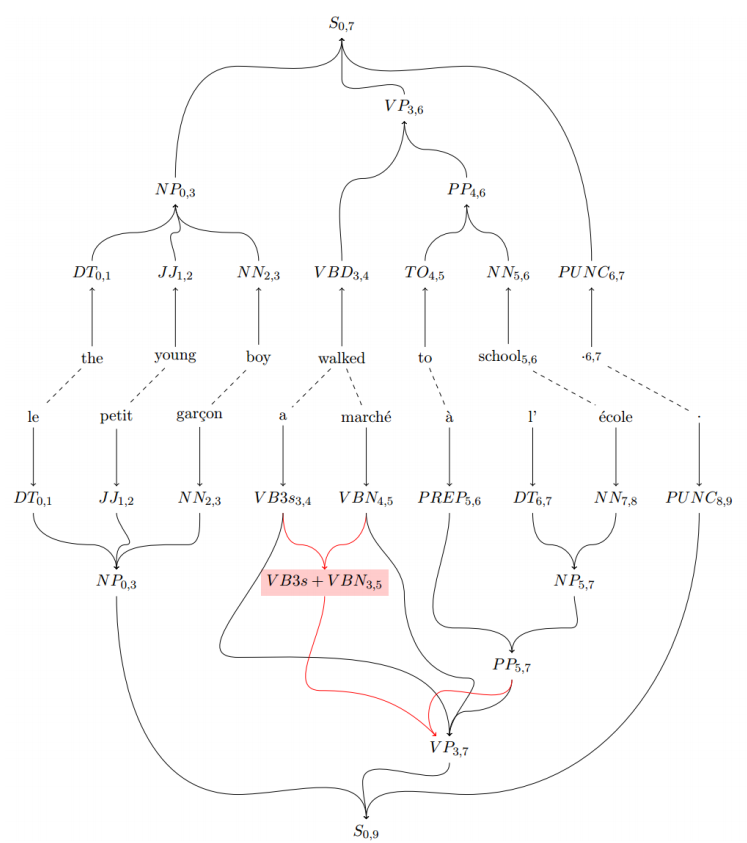
\includegraphics[scale=0.25]{virtualnode.png}
\caption{A pair of aligned trees, turned into hypergraphs. Non-terminal symbols are annotated with their half-open spans. \texttt{NP}$_{0,3}$ represents an \texttt{NP} over the span $[0,3)$.
An example virtual node and its corresponding virtual edges is shown in red.}
\label{virtualnodefig}
\end{figure}

The next step of the rule extraction process is to find pairs of aligned nodes in the hypergraphs.
We will call a source node $S$ and a target node $T$ \emph{node-aligned} if the following conditions hold.
First, if $S$ and $T$ must either both be non-terminals or both be terminals.
Aligning a terminal to a non-terminal or vice-versa is disallowed.
Second, there must be at least one alignment link from a terminal dominated by $S$ to a terminal dominated by $T$.
Third, there must be no alignment links from terminals dominated by $S$ to terminals outside of $T$ or vice-versa.

We define a ``rule'' to be pair of hyperedges whose heads are node-aligned as per the above definition,
and whose non-terminal children are node-aligned in a one-to-one manner.
For example, in the sample tree, we see that the source node \texttt{PP}$_{4,6}$ is
node-aligned to the target node \texttt{PP}$_{5,7}$. Furthermore, their children are also node-aligned
one-to-one: \texttt{TO}$_{4,5}$ to \texttt{PREP}$_{5,6}$ and \texttt{NN}$_{5,6}$ to \texttt{NP}$_{5,7}$.
Thus this pair of edges will give rise to the rule \texttt{[PP::PP]} $\rightarrow$ \texttt{[TO,1] [NN,2] ||| [PREP,1] [NP,2]}.
Note that since there are no edges headed by terminals, so will not extract any rules with terminal heads.

The above formulation allows the extraction of minimal rules that do not skip any internal structure, but does not yet
include any mechanism for extracting \emph{composed} rules, which may skip levels of internal structure.
To capture such rules, we first pre-process each input hypergraph, recursively adding hyperedges from non-overlapping sets
of descendent nodes. For example, one hyperedge we add to the source side of the sample hypergraph pair is
\texttt{VP}$_{3,6}$ $\rightarrow$ \texttt{walked TO}$_{4,5}$ NN$_{5,6}$. Independently, on the target side we add an edge
\texttt{VP}$_{3,7}$ $\rightarrow$ \texttt{a march\'{e} PREP}$_{5,6}$ NP$_{5,7}$.

Now when we extract rules, we will find these two edges to be corresponding -- their heads are node-aligned, and their non-terminal
tails are also node-aligned one-to-one. Thus these two edges will combine to give the rule
\texttt{[VP::VP]} $\rightarrow$ \texttt{walked [TO,1] [NN,2] ||| a march\'{e} [PREP,1] [NP,2]}, a composed rule not extractable
by the bald algorithm.

While using composed edges allows us to extract all permissible rules from a pair of aligned trees, to be consistent with previous work,
we introduce one more type of hypergraph augmentation.
\citet{hanneman2011general} allow for adjacent sibling non-terminal nodes to be merged into one \emph{virtual node}, which may then be node-aligned to opposite nodes,
be they ``real'' or virtual. To enable this, we explicitly add virtual nodes to our hypergraph and connect them to their children with a hyperedge.
Furthermore, for every hyperedge that contained all of the sibling nodes
as non-terminal tails, we add a duplicate hyperedge that uses the new virtual node instead. For example, in Fig.~\ref{virtualnodefig},
we have added a new non-terminal node labeled \texttt{VB3s+VBN}$_{3,5}$ to the hypergraph. This node represents the fusion of the \texttt{VB3s}$_{3,4}$ and \texttt{VBN}$_{4,5}$ nodes.
We then add a hyperedge headed by the new \texttt{VB3s+VBN}$_{3,5}$ with tails to both \texttt{VB3s}$_{3,4}$ and \texttt{VBN}$_{4,5}$.
Furthermore, we make a copy of the edge \texttt{VP}$_{3,7}$ $\rightarrow$ \texttt{VB3s}$_{3,4}$ \texttt{VBN}$_{4,5}$ \texttt{PP}$_{5,7}$, and replace the
\texttt{VB3s}$_{3,4}$ and \texttt{VBN}$_{4,5}$ tail nodes with a single tail, \texttt{VB3s+VBN}$_{3,5}$, to form the new edge
\texttt{VP}$_{3,7}$ $\rightarrow$ \texttt{VB3s+VBN}$_{3,5}$ \texttt{PP}$_{5,7}$. The addition of this new hyperedge allows the extraction of the rules
\texttt{[VBD::VB3s+VBN]} $\rightarrow$ \texttt{walked ||| a march\'{e}} and
\texttt{[VP::VP]} $\rightarrow$ \texttt{[VBD,1] [PP,2]  ||| [VB3s+VBN,1] [PP,2]}, both of which were unextractable without the virtual node.

With the addition of virtual nodes, our work is directly comperable to \citet{hanneman2011general}, while being more modular, extensible and provably correct.
One particularly interesting extension our hypergraph formulation allows is the use of weighted parse \emph{forests} rather than $1$-best trees.
This helps our rule extractor to overcome parser errors and allows us to easily handle cases of ambiguity, in which two or more trees may be equally likely
for a given input sentence. In Section~\ref{sec:experiments} we will show that this ability alone can add up to +1.1 \textsc{BLEU} \cite{papineni2002bleu} in a Chinese--English system.

\section{Experiments}
\label{sec:experiments}
We tested our rule learner on the FBIS Chinese--English corpus (LDC2003E14), which consists of 302,966 sentence pairs or 9,350,506 words on the English side.
We first obtain $k$-best parses for both sides of FBIS using the Berkeley Parser\footnote{https://code.google.com/p/berkeleyparser/} and align the corpus using \texttt{fastalign} \cite{dyer-chahuneau-smith:2013:NAACL-HLT}.
We use a 5-gram language model built with KenLM \cite{heafield2011kenlm} on version four of the English GigaWord corpus plus the target side of FBIS, smoothed with improved Kneser-Ney smoothing \am{kneser1995improved}.
For each set up we extract rules using \texttt{grex} \cite{hanneman2011general} or our new tool.
When using our tool we have the option of simply using $1$-best trees to compare directly to \texttt{grex}, or using the weighted forests consisting of all of Berkeley's $k$-best parses on
the source side, the target side, or both. For these experiments we use $k=10$.
Each system is tuned on mt06 using Hypergraph MERT \cite{kumar2009efficient} towards BLEU.
We then test each system on both mt03 and mt06, evaluting with MultEval \cite{clark2011better}, which calculates BLEU, METEOR \cite{denkowski2011meteor}, and TER \cite{snover2006study}.

Details concerning the size of the extracted grammars can be found in Table \ref{grammarsizes}.
Translation quality results are shown in Table \ref{bleuresults}.

\begin{figure}[ht!]
\centering
\begin{tabular}{r c c c c c}
Extractor & $k_s$ & $k_t$ & Instances & Types & Avg. Sent. Grammar \\
\hline
\texttt{grex} & 1 & 1 & 24.9M\footnote{This indicates that \\texttt{grex} failed to extract certain valid rules. This conclusion was validated by our team, and confirmed with the authors of \cite{hanneman2011general}.} & 11.8M & 210K \\
\texttt{HyperGrex} &  1 &  1 & 25.9M & 12.7M & 240K \\
\texttt{HyperGrex} &  1 & 10 & 33.3M & 17.7M & 398K \\
\texttt{HyperGrex} & 10 &  1 & 33.7M & 17.9M & 397K \\
\texttt{HyperGrex} & 10 & 10 & 48.7M & 24.3M & 541K \\
\end{tabular}
\caption{Grammar sizes using different grammar extraction set ups.
$k_s$ ($k_t$) represents the number of source (target) trees used.}
\label{grammarsizes}
\end{figure}

\begin{figure}[ht!]
\centering
\begin{tabular}{r c c c c c}
Extractor & $k_s$ & $k_t$ & mt06 & mt03 & mt08 \\
\texttt{grex}      &  1 &  1 & 29.6 & 31.8 & 23.4 \\
\texttt{HyperGrex} &  1 &  1 & 30.1 & 32.4 & 24.0 \\
\texttt{HyperGrex} &  1 & 10 & \textbf{30.4} & \textbf{32.9} & \textbf{24.3} \\
\texttt{HyperGrex} & 10 &  1 & 29.5 & 32.0 & 23.1 \\
\texttt{HyperGrex} & 10 & 10 & 30.0 & 32.7 & 23.7 \\
\end{tabular}
\caption{\textsc{BLEU} results on mt06 (tuning set), mt03, and mt08 using various grammar extraction configurations.}
\label{bleuresults}
\end{figure}

\section*{Acknowledgements}
This research is supported by \ldots

\bibliography{mtm2014}

\correspondingaddress
\end{document}
